\subsection{TOF}
\subsubsection{Introduction}

Differently from other sub-systems, namely the ITS and the TPC that have been deeply renewed during LS2,  the TOF upgrade involved mainly part of its readout electronics. Nevertheless also this upgrade programme is intended to allow the TOF to accomplish a continuous readout during Run3 data taking, aligning with ITS and TPC, and with the aim to exploit at maximum its particle identification discriminating power in the intermediate momentum range. The intervention needed to adapt to a continuous readout was relatively limited thanks to the intrinsic deadtime of the Multi-gap Resistive-Plate Chamber (MRPC) detector and its front-end electronics, which is very low ($\approx$10 ns)). The second key element contributing to design a relatively small intervention was the existing on-board buffering resources for digitized data, already available via the architecture of the High Performance TDC (HPTDC), as detailed in the next sub-section. 

\subsection{Implementation of continuous readout}
The ALICE Time-Of-Flight (TOF) detector~\cite{TOF1,TOF2} is a large array of 1593 Multi-gap Resistive-Plate Chamber (MRPC) strip detectors organized in supermodules covering the 18 sectors of the ALICE spaceframe. Each of the sectors is read out by four VME custom crates, each hosting 9 or 10 TDC Readout Module (TRM) boards, one Data Readout Module (DRM) card acting as master and having interfaces with central systems, and one card named Local Trigger Module (LTM). that elaborates trigger information and set the threshold on the NINO ASIC chips hosted on the Front-End cards.

The TRM cards are equipped with 30 High Performance TDC (HPTDC) operated in very high resolution mode, with 24.4 ps LSB. The specifications of the HPTDC (and its perfomance once integrated in the TRM cards) is detailed elsewhere~\cite{Akindinov:2004gf}, but it is important to recall here its trigger matching function. Based on time tags, the HPTDC allows the trigger latency to be programmable over a large dynamic range and also ensures the capability of supporting overlapping triggers, where individual hits may be assigned to multiple events. Once a trigger is received, only stored hits starting from a given latency time and for a limited matching window are moved to the readout FIFO and made ready for further stages of readout. During Run1 and Run2, with a limited high-rate capacity in the barrel detectors of ALICE (given intrinsic limitations of the TPC with a readout based on multiwire proportional chambers and a gating grid to block ion backflow) the trigger was limited to few kHz. In such a scheme for the TOF the internal HPTDC buffers were set with a latency window of 6500 ns (corresponding to the latency of the triggers reaching the TOF crates) and with a matching window of 600 ns, able to collect comfortably all hits registered in the TOF detector associated to that trigger.

\begin{figure}[b!]
\centering
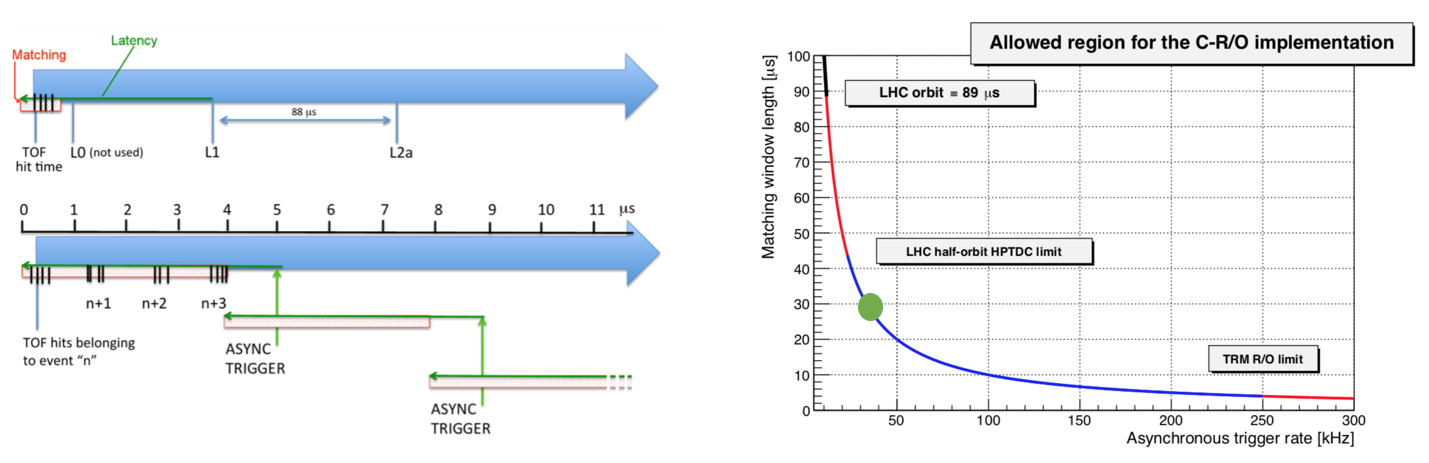
\includegraphics[width=1.0\textwidth]{tofCR.png} 
\caption{(left) HPTDC programming in Run1/Run2 operations (top arrow) and in Run3 (bottom arrow), mimicking a continuous readout. All hits are readout and hits registered (black lines) are later associated to physical events. (right) Possible selection of parameters (fixed trigger frequency and matching window width) to realize a continuous readout. The green circle corresponds to the chosen point of operations.}
\label{fig:cro}
\end{figure}

Provided certain conditions are respected, it is possible to use this setup to mimic a continuos readout. Actually when a strictly periodic trigger, typically at fixed bunch crossing, is delivered with a certain frequency $f_T$ and a matching window $m_w$ is set, if the condition $f_{T} \times m_{w} = 1 $ is satisfied, the system will readout all hits. In Fig.~\ref{fig:cro}(left) the basic idea is represented. Delivering a trigger with a constant 50 kHz frequency, and setting latency and matching windows of 20 $\mu$s, all hits are read-out. In Fig.1~\ref{fig:cro}(right) the curve of allowed values is represented, together with the limitations of the system. From one side the latency window cannot be set at value larger than half of a LHC orbit. On the other hand, as discussed in the ALICE Readout Upgrade TDR~\cite{Antonioli:2013ppp}, the trigger frequency cannot be too high, given the time spent reading the HPTDC chains in the TRM cards (they host 2 HPTDC chains of 15 chips, with a fixed 3.2 $\mu$s readout deadtime just for token-passing operations among chips. More generally the readout time $T_{readout}$ has to be less than $1/f_{T}$). Considering also the readout time over the VME backplane (up to 10 TRMs per crate have to be read) an optimization point was found with a 33 kHz periodic trigger.  A real and full ``simulation'' in the lab was completed, sending random hits to several TRM cards, programmed with appropriate latency and matching windows (29800 ns) and TOF special triggers (TT) delivered at fixed bunch crossing (the orbit is split in three parts with TT occurring at BC\#: 51, 1177 and 2673). Fig.~\ref{fig:hits} shows no hits were lost (given their random distribution they are expected to be distributed with equal probabiity along the LHC orbit).

\begin{figure}[t!]
\centering
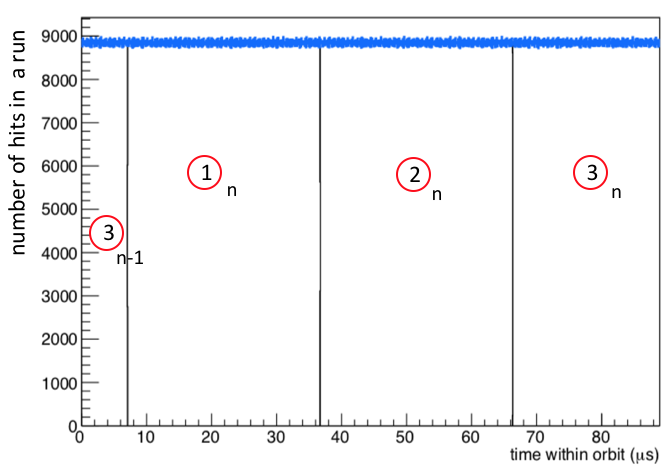
\includegraphics[width=0.6\textwidth]{hits.png} 
\caption{Hit time of randomized hits sent at fixed rate to HPTDC inside a TOF crate operated in continuous readout mode. Subsequent orbits are overlapped in the plot. All bunch crossing are covered, spanning through the whole LHC orbit.}
\label{fig:hits}
\end{figure}


\subsubsection{The new Data Readout Module (DRM2)}
In order to cope with the planned increase of luminosity and of the interaction rate (up to 1 MHz in proton-proton collisions and 50 kHz in lead-lead collisions), a new board, named Digital Readout Module 2 (DRM2), was designed. With respect to the existing DRM module (hereafter DRM1) it has more modern FPGA (Microsemi IGLOO2) and, overall, it replaces the Run1/Run2 links towards the DAQ based on the DDL and TTC projects. The card features a faster link towards the data acquisition system using the GBTx ASIC~\cite{GBTx} and VTRx optical transceiver~\cite{VTRX} from CERN, allowing a user bandwidth towards the Data AcQuisition system (DAQ) of 3.2 Gb/s. As anticipated in its final configuration the readout is implemented with synchronous triggers at fixed bunch crossing values at 33 kHz, setting a matching window of 30 microseconds in the HPTDC installed in the TRMs. As explained, this solution mimics a full-fledged continuous readout as all ALICE detector upgraded readout chains. The same link is also used for receiving triggers and a low-jitter clock, which can be distributed to the front-end electronics as primary clock. For the TOF detector the quality of this clock is crucial and a campaign of measurements on the clock received from the ALICE data acquisition card named CRU (Common Readout Unit) has been carried out: we measured a RMS clock jitter as low as $\approx$10 ps in the laboratory, which is compatible with the requirements. A devoted line of clock distribution of the LHC clock is, however, in place as it was during Run1 and Run2 with a similar jitter.

\begin{figure}[t!]
\centering
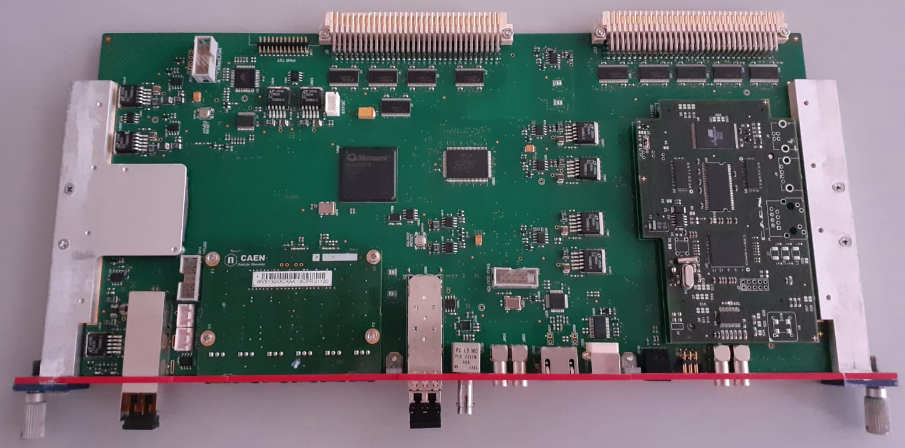
\includegraphics[width=0.6\textwidth]{drm2.png} 
\caption{The DRM2 card: on the left the VTRX transceiver and the GBTx ASIC (covered by a heat dissipating panel). On the right it is visible the ARM piggy-back card. The additional optical receivers for the SCL and the LHC clock (see text) are also visible.}
\label{fig:drm2}
\end{figure}


A picture of the DRM2 card~\cite{Falchieri:2018fqw} is shown in Fig.~\ref{fig:drm2}. It is a narrow 9U VME card (16 cm x 33 cm) with the same form factor as the DRM1 and the TRM boards. The heart of the board is a Microsemi Flash-based IGLOO2 FPGA, (M2GL090-FG676 with silicon revision 3) which drives the trigger and data flows inside the crate. This device has been chosen since the expected TID (Total Ionizing Dose) for the board (placed at $\approx$4 meters far from the beam pipe) is 0.13 krads in 10 years, which is acceptable for such a device. The advantage is that the FPGA configuration memory is SEU (Single Event Upset) immune, so that scrubbing is not needed. Results of irradition tests on several components of the DRM2, including the IGLOO2 FPGA, commercial optical transceivers, and staging RAM were reported in~\cite{Falchieri:2019ulw}.

The FPGA – GBTx connection consists of a single 40-bit large parallel lane of 80 MHz differential signals. The same configuration was previously tested on a GBTx test board developed before designing the DRM2: we could measure a BER lower than $10^{-14}$ and a total jitter on the received clock around 50 ps~\cite{Falchieri:2017ofi}. As in DRM1 an additional optical link (SCL: Slow Control Link) is implemented, providing a firmware implementation of CONET2 protocol developed by CAEN~\cite{CONET2}. All DRM2 are actually connected to commercial A3818 PCIe cards, housed in Linux machines hosted in the DCS network. The SCL is used for configuration of the front-end electronics and programming of all VME cards. In addition, while the data collected are immediately sent to central DAQ via the GBTx link, the firmware also store them in the staging RAM (1Mx36 bit SSRAM from Cypress: CY7C1460KV33). Data are then transferred (1 MB buffers) to the DCS machines. From data, some values as temperatures are stripped and reported in the DCS via DIM servers. In addition Quality Control programs run on these data. The SCL has therefore a dual role: configuration and monitoring.

A block of hardware inherited by DRM1 is the ARM microprocessor mounted on A1500 provided by CAEN. This CPU implements, via JTAG over the VME backplane, the programming of Actel APA750 and APA600 installed in TRM and LTM cards respectively. The connection on the front panel to the consolle port of this CPU was improved, with respect to the DRM1, using a commercial RS232-USB interface (and it is therefore easily pluggable via USB cable from laptops). The ARM CPU is also able to program the firwmare of the IGLOO2 FPGA. As for the A1500 mounted on the DRM1, thanks to the modified Ethernet interface (validated to operate also in magnetic field) all the firmware updates of the VME cards can be remotely executed.

Finally the DRM2 distributes the clock to all VME cards inside the crate. This is an entirely new functionality with respect to Run1 and Run2 configuration. Previously only every two crates TOF had a clock distribution module (Clock and Pulse Distribution Module, CPDM), and this created some tricky dependency in the power-up and configuration sequences, as well as a not desirable higher concentration of single points of failures (given that if a power supply fails on the crate hosting the CPDM, also the second crate was not usable given clock was not distributed). The DRM2 in a user-selectable way can distribute to all cards hosted in its VME crate a local clock, the clock received via GBTx and the clock received directly from the LHC interface. For the latter an optical receiver from PD-LD/NECSEL, with ST plug-type, with pinout compatible with the Truelight TRR-1B43-000 previously widely used for TTC applications. This latter configuration will minimize the jitter of the clock distributed to TRM cards.


All the DRM1 were removed and disassembled during the first months of 2019, with A1500 ARM piggy-back cards tested and prepared for installation on DRM2. The procedure for validation and test of the production of DRM2 (completed during 2019) was described in~\cite{Falchieri:2019mpp}. The installation of all DRM2 cards, partially delayed by the pandemic, was ended in June 2020 with commissioning now well underway. All 72 TOF crates have already taken data via the GBTx interface, with data sent to CRU and FLP. 


\subsubsection{Other systems}
During the LS2, several other TOF systems were, in addition to the readout part, subject to key improvements and maintenance, preparing for the intense data taking foreseen in RUN3. Among many interventions, we highlight in particular:
\begin{itemize}
\item the DC/DC systems (CAEN modules A1395 and A1396): these modules are responsibile of power supply for the four crates of each TOF supermodules. They receive a DC 48V power supply via bus-bars from outside the L3 Magnet and provide LV power supply for VME boards and Front-end cards on MRPC modules. A solid state fuse that was subject to frequent breakdown was replaced. Additionally a study via proton irradiation at Centro di Protonterapia in Trento in 2019 investigated the cause of SEU events, registered in 2018 at high irradiation rate, and that produced sudden loss of communication with the module. The addition of a filter capacity on the reset line of the microprocessor on the A1396 fixed the problem. A full refurbishment of all modules (entailing dismounting 216 modules from the detector) was completed in 2019-2020.
\item all DRM2 are equipped with an ARM microprocessor (AT91RM9200 from Atmel) running Linux. During Run1 and Run2 these CPUs were used exclusively to perform firmware upgrades on VME boards via JTAG interface on VME backplane using Actel software for APA FPGAs. Using the cross-platform development tools provided, it has been now deployed a full running  slow control DIM server on these CPUs that will provide an additional channel to monitor voltages and temperature on the cards (even if the Slow Control Link is not connected). More importantly, thanks to a different hardware implementation on DRM2 with respect to DRM1, via the server running on ARM CPUs it will be possible: i) to reset the CONET link; ii) to reset the Microsemi FPGA of the DRM2. These two emergency resets are planned to be used in case of loss of communication with the DRM2 (on the SCL), without the need of executing a power cycle. This will be useful especially because now the DRM2 provides the primary clock to all TRM cards and a DRM2 power cycle would cause the loss of the clock and therefore the need of a power cycle in all VME slots in the crate.
\item The procedure for the control and validation of the recorded data has been integrated into the O2 framework under the project of the Quality Control (QC).
The new QC system merges in one the Quality Assurance (QA) and Data Quality Monitoring, these were kept separate during Run2. The aim of data QC spy on the flow of data is to give useful information on the quality of the data being recorded.
The QC is also responsible for oversee the processes underlying the handling and transformation of this data, such as reconstruction and calibration. The QC has been developed to provide a detailed insight into the various steps of the data processing (e.g. raw data, digits). This setup will be used on the dedicated computing nodes (FLPs/EPNs) to monitor the TOF data stream as well as in the TOF DCS cluster, sampling data through the SCL, as mentioned before.
\item The data flow from the CRUs is processed by the FLP CPUs with the goal of performing the first level of data decoding and manipulation (preprocessing). The preprocessing produces a second-level of raw data that provides a zero-suppressed data stream where the relevant information stored in a compact format and prepared for next stage timeframe analysis. This effectively reduces the output bandwidth from the FLP to the EPNs by a significant amount (a factor 4x at saturation for very-high multiplicity events, a much larger factor for low-multiplicity events) and allows the framework to make the best use of the available computing resources on the FLP by performing low-level data monitoring. The QC system is able to access the preprocessed data directly on the FLPs for monitoring the raw data stream as early as possible.
\end{itemize}
